\subsection{Chi tiết các bảng}
    \begin{table}[h!]
      \centering
      \begin{tabular}{|l|p{0.3\textwidth}|c|c|c|}
        \hline
        \textbf{Thuộc tính} & \textbf{Diễn giải} & \textbf{Kiểu dữ liệu} & \textbf{PK} & \textbf{FK}\\
        \hline
        id & mã số sinh viên & char & X &\\
        \hline
        full\_name & tên sinh viên & char & &\\
        \hline
        gender & giới tính & bit & &\\
        \hline
        cpa & điển trung bình & int & &\\
        \hline
        school\_credit\_debt & số tín chỉ nợ & int & &\\
        \hline
        school\_credit\_complete & số tin chỉ đã hoàn thành & int & &\\
        \hline
        user\_id & mã tài khoản & int & & X\\
        \hline
      \end{tabular}
      \caption{Bảng sinh viên}
    \end{table}

    \begin{table}[h!]
      \centering
      \begin{tabular}{|l|p{0.45\textwidth}|c|c|c|}
        \hline
        \textbf{Thuộc tính} & \textbf{Diễn giải} & \textbf{Kiểu dữ liệu} & \textbf{PK} & \textbf{FK}\\
        \hline
        id & mã CV & int & X &\\
        \hline
        summary & giới thiệu bản thân & text & &\\
        \hline
        skill & kỹ năng của sinh viên & text &  &\\
        \hline
        education & trình độ học vấn & text & &\\
        \hline
        activity & hoạt động ngoại khoá & text & &\\
        \hline
        experience & kinh nghiệm & text & &\\
        \hline
        project & các dự án đã tham gia & text & &\\
        \hline
        student\_id & mã sinh viên & char & & X\\
        \hline
      \end{tabular}
      \caption{Bảng CV}
    \end{table}

    \begin{table}[h!]
      \centering
      \begin{tabular}{|l|p{0.45\textwidth}|c|c|c|}
        \hline
        \textbf{Thuộc tính} & \textbf{Diễn giải} & \textbf{Kiểu dữ liệu} & \textbf{PK} & \textbf{FK}\\
        \hline
        id & mã lớp & int & X &\\
        \hline
        full\_name & tên lớp & char & &\\
        \hline
        major\_id & mã ngành & char & & X\\
        \hline
        lecturer\_id & mã giảng viên phụ trách & int & & X\\
        \hline
      \end{tabular}
      \caption{Bảng lớp sinh viên}
    \end{table}

    \begin{table}[h!]
      \centering
      \begin{tabular}{|l|p{0.45\textwidth}|c|c|c|}
        \hline
        \textbf{Thuộc tính} & \textbf{Diễn giải} & \textbf{Kiểu dữ liệu} & \textbf{PK} & \textbf{FK}\\
        \hline
        id & mã ngành & char & X & \\
        \hline
        full\_name & tên ngành & char & &\\
        \hline
        institute\_id & mã viện & char &  & X\\
        \hline
      \end{tabular}
      \caption{Bảng ngành học}
    \end{table}

    \begin{table}[h!]
      \centering
      \begin{tabular}{|l|p{0.45\textwidth}|c|c|c|}
        \hline
        \textbf{Thuộc tính} & \textbf{Diễn giải} & \textbf{Kiểu dữ liệu} & \textbf{PK} & \textbf{FK}\\
        \hline
        id & mã viện & char & X &\\
        \hline
        full\_name & tên viện & char & &\\
        \hline
      \end{tabular}
      \caption{Bảng viện đào tạo}
    \end{table}

    \begin{table}[h!]
      \centering
      \begin{tabular}{|l|p{0.45\textwidth}|c|c|c|}
        \hline
        \textbf{Thuộc tính} & \textbf{Diễn giải} & \textbf{Kiểu dữ liệu} & \textbf{PK} & \textbf{FK}\\
        \hline
        id & mã tài khoản người dùng & int & X &\\
        \hline
        username & tên đăng nhập & char & &\\
        \hline
        email\_school & email trường cấp & char & &\\
        \hline
        email\_other & email cá nhân & char & &\\
        \hline
        facebook\_link & đường dẫn liên kết với mạng xã hội người dùng & char & &\\
        \hline
        role & phân quyền (0 - admin; 1 - giảng viên; 2 - sinh viên) & tinyint & &\\
        \hline
      \end{tabular}
      \caption{Bảng người dùng}
    \end{table}

    \begin{table}[h!]
      \centering
      \begin{tabular}{|l|p{0.45\textwidth}|c|c|c|}
        \hline
        \textbf{Thuộc tính} & \textbf{Diễn giải} & \textbf{Kiểu dữ liệu} & \textbf{PK} & \textbf{FK}\\
        \hline
        id & mã giảng viên & int & X &\\
        \hline
        full\_name & tên giảng viên & char & &\\
        \hline
        gender & giới tính & bit & &\\
        \hline
        user\_id & mã tài khoản & int & & X\\
        \hline
      \end{tabular}
      \caption{Bảng giảng viên}
    \end{table}

    \begin{table}[h!]
      \centering
      \begin{tabular}{|l|p{0.45\textwidth}|c|c|c|}
        \hline
        \textbf{Thuộc tính} & \textbf{Diễn giải} & \textbf{Kiểu dữ liệu} & \textbf{PK} & \textbf{FK}\\
        \hline
        id & mã chủ đề & int & X &\\
        \hline
        full\_name & tên chủ đề & char & &\\
        \hline
        description & mô tả chi tiết & text & &\\
        \hline
        major\_id & mã ngành & char & & X\\
        \hline
        lecturer\_id & mã giảng viên & int & & X\\
        \hline
      \end{tabular}
      \caption{Bảng chủ đề nghiên cứu đồ án}
    \end{table}

    \begin{table}[h!]
      \centering
      \begin{tabular}{|l|p{0.4\textwidth}|c|c|c|}
        \hline
        \textbf{Thuộc tính} & \textbf{Diễn giải} & \textbf{Kiểu dữ liệu} & \textbf{PK} & \textbf{FK}\\
        \hline
        id & mã thông tin & int & X &\\
        \hline
        full\_name & tên thực tập & char & &\\
        \hline
        name\_company & tên công ty thực tập & char & &\\
        \hline
        address\_company & địa chỉ công ty & char & &\\
        \hline
        description & mô tả chi tiết nội dung thực tập & text & &\\
        \hline
        lecturer\_id & mã giảng viên & int & & X\\
        \hline
      \end{tabular}
      \caption{Bảng thông tin thực tập}
    \end{table}

    \begin{table}[h!]
      \centering
      \begin{tabular}{|l|p{0.45\textwidth}|c|c|c|}
        \hline
        \textbf{Thuộc tính} & \textbf{Diễn giải} & \textbf{Kiểu dữ liệu} & \textbf{PK} & \textbf{FK}\\
        \hline
        id & mã đơn & int & X &\\
        \hline
        student\_id & mã sinh viên đăng ký & char & & X\\
        \hline
        semester & học kỳ (1 , 2, 3 - kì hè) & tinyint & &\\
        \hline
        time\_register & thời gian gửi đơn đăng ký & datetime & &\\
        \hline
      \end{tabular}
      \caption{Bảng đơn đăng ký đồ án}
    \end{table}

    \begin{table}[h!]
      \centering
      \begin{tabular}{|l|p{0.4\textwidth}|c|c|c|}
        \hline
        \textbf{Thuộc tính} & \textbf{Diễn giải} & \textbf{Kiểu dữ liệu} & \textbf{PK} & \textbf{FK}\\
        \hline
        id & mã đơn chi tiết & int & X &\\
        \hline
        form\_id & mã đơn & int & & X\\
        \hline
        status\_contact & trạng thái liên hệ với giảng viên (0 - chưa liên hệ; 1 - đã liên hệ) & bit & &\\
        \hline
        status\_check & trạng thái duyệt đơn & bit & &\\
        \hline
        topic\_orientation & định hướng chủ đề & char & &\\
        \hline
        type\_project & loại đồ án (1 - toán cơ bản, 2 - toán ứng dụng, 3 - toán-tin, ...) & tinyint & &\\
        \hline
        desired\_order & thứ tự nguyện vọng (1, 2, 3) & tinyint & &\\
        \hline
        lecturer\_id & mã giảng viên & int & & X\\
        \hline
      \end{tabular}
      \caption{Bảng chi tiết đơn đăng ký đồ án}
    \end{table}

    \begin{table}[h!]
      \centering
      \begin{tabular}{|l|p{0.4\textwidth}|c|c|c|}
        \hline
        \textbf{Thuộc tính} & \textbf{Diễn giải} & \textbf{Kiểu dữ liệu} & \textbf{PK} & \textbf{FK}\\
        \hline
        id & mã đơn & int & X &\\
        \hline
        student\_id & mã sinh viên đăng ký & char & & X\\
        \hline
        semester & học kỳ (1, 2, 3 - kì hè) & tinyint & &\\
        \hline
        time\_register & thời gian gửi đơn đăng ký & datetime & &\\
        \hline
        lecturer\_id & mã giảng viên & int & & X\\
        \hline
        status\_contact & trạng thái liên hệ với giảng viên (0 - chưa liên hệ; 1 - đã liên hệ) & bit & &\\
        \hline
        status\_check & trạng thái duyệt đơn & bit & &\\
        \hline
      \end{tabular}
      \caption{Bảng chi tiết đơn đăng ký thực tập}
    \end{table}

\subsection{Biểu đồ dữ liệu quan hệ}
\begin{landscape}
  \begin{center}
    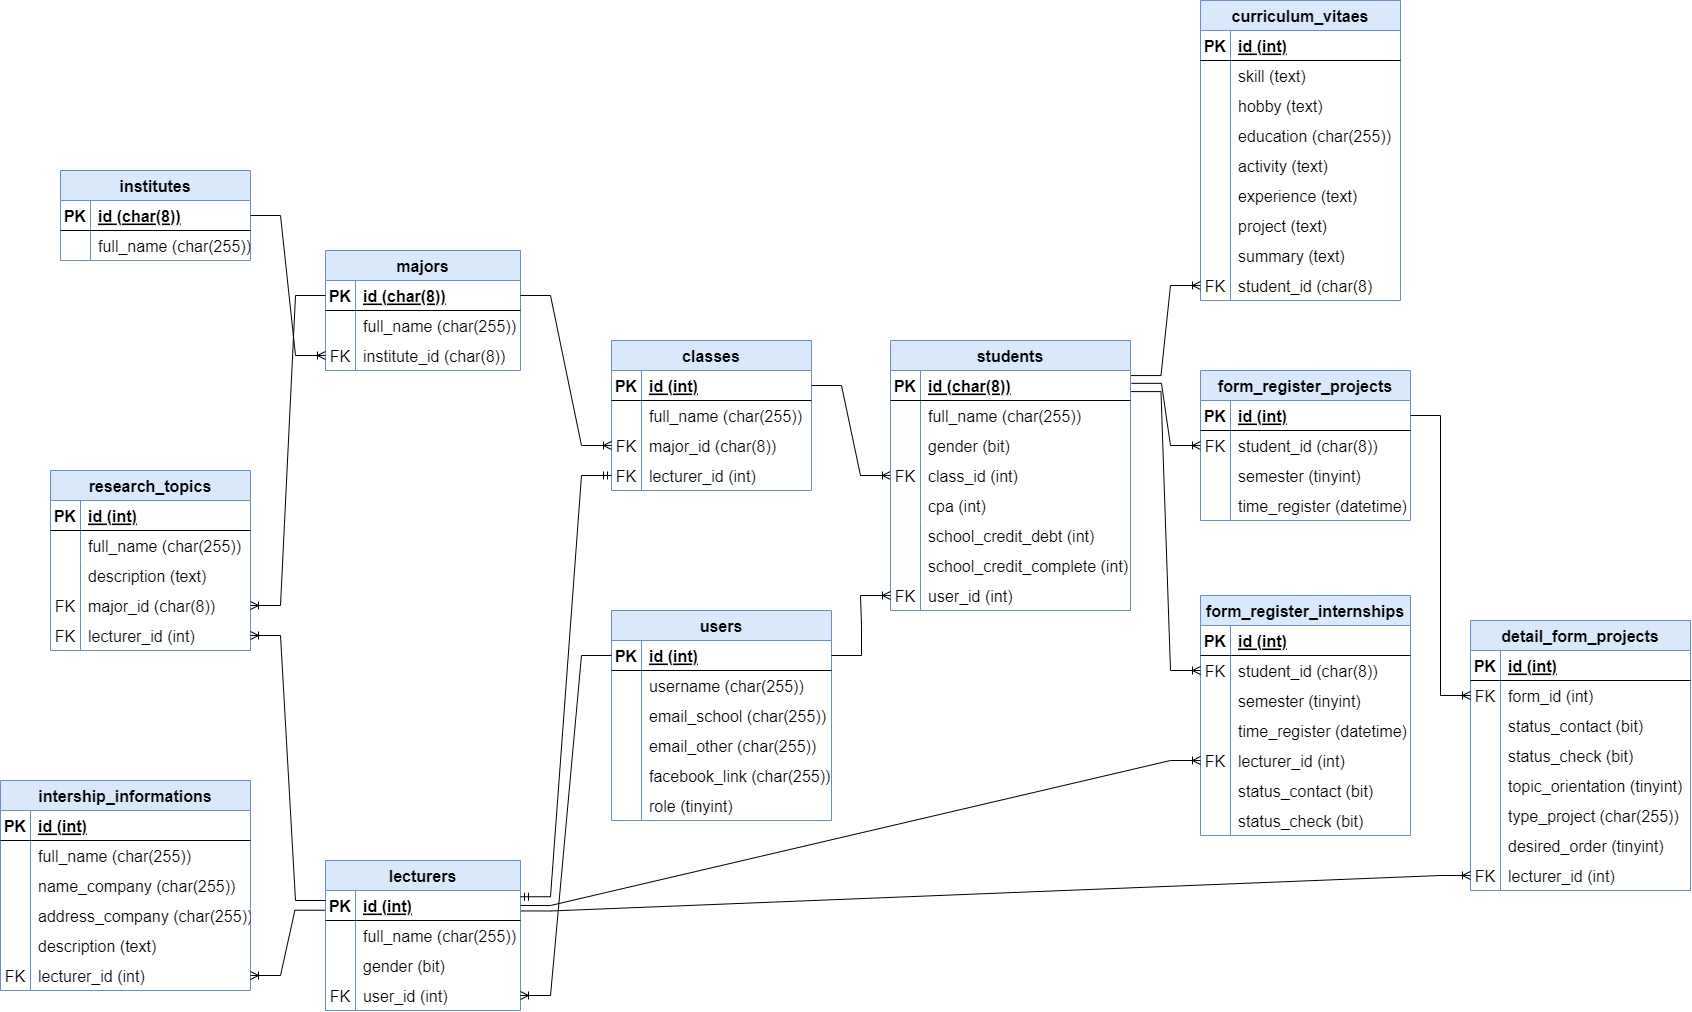
\includegraphics[width=1.5\textwidth]{../drawio/db_sv11.png}
    \begin{figure}[h]
      \centering
      \caption{Biểu đồ dữ liệu quan hệ}
    \end{figure}
  \end{center}
\end{landscape}